\documentclass[../main.tex]{subfiles}
\graphicspath{{\subfix{../../images/}}}

\begin{document}

The von neumann architecture specifies a generic structure for CPUs and microprocessors to follow when they are designed. It dictates that the data used to store programs and the data used by the program (tempoary values, variables in memory) should co-exist in the same memory.

The following is a diagram of the von neumann architecture:

\begin{figure}[H]
    \centering
    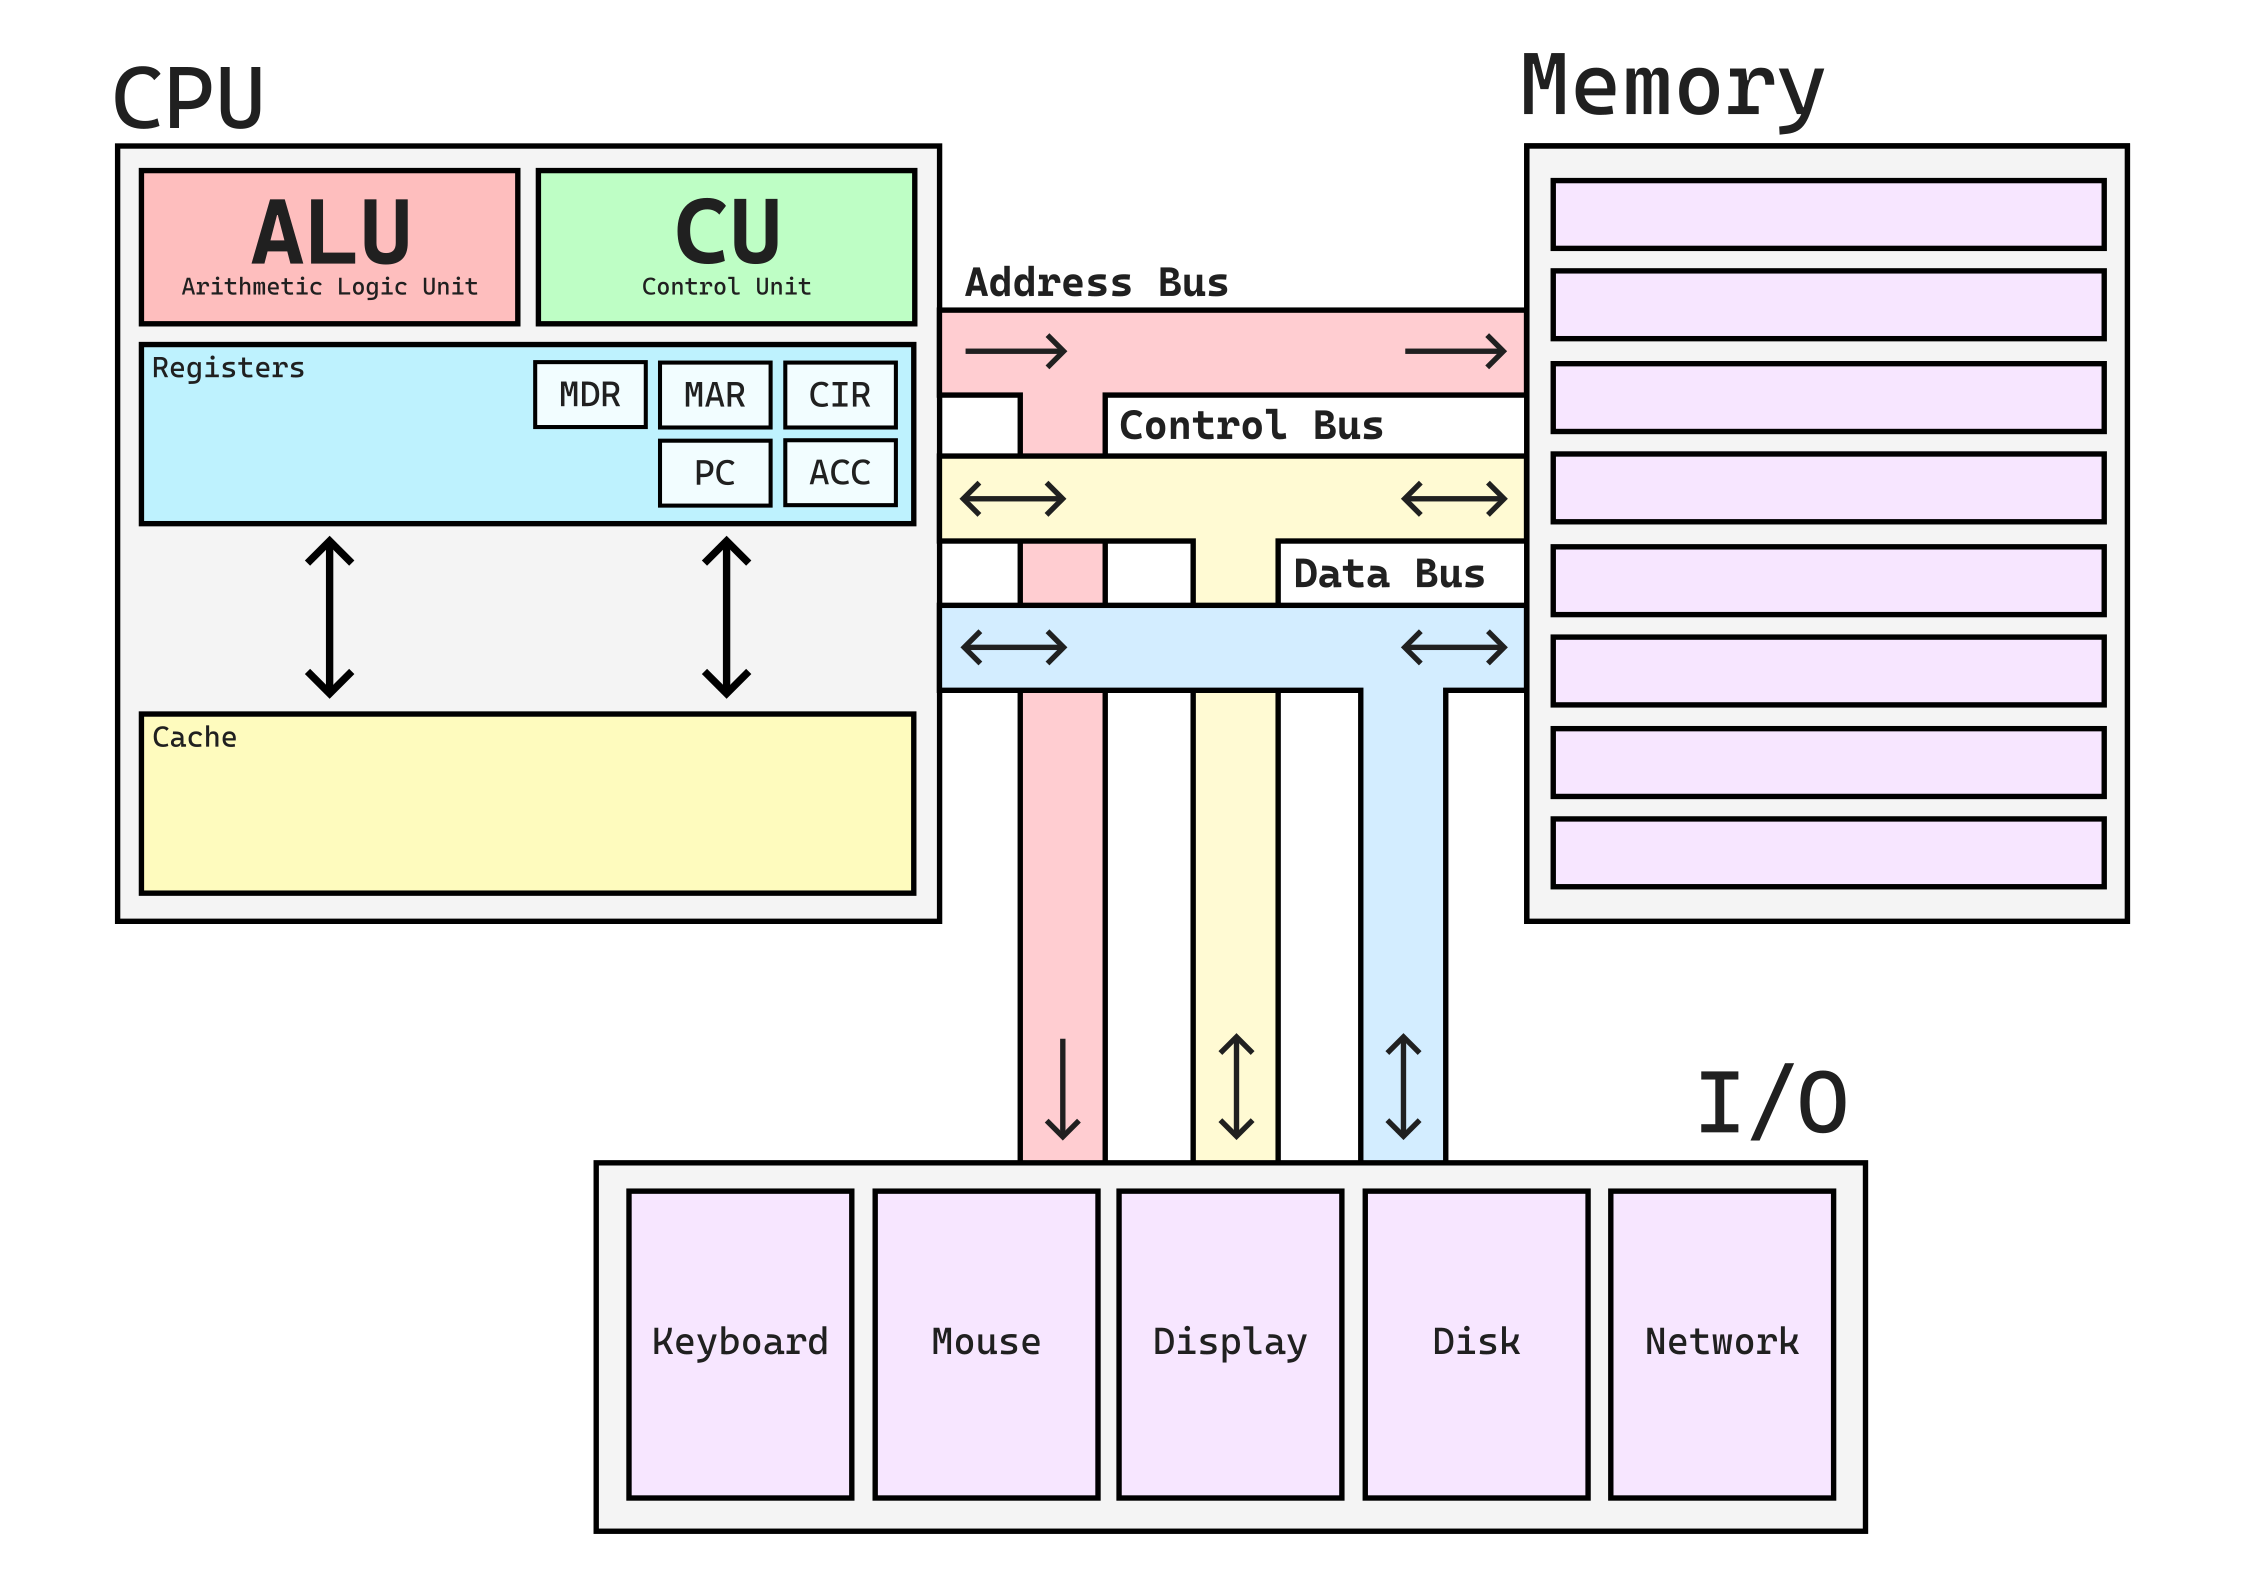
\includegraphics[width=0.85\textwidth]{vonneumann.png}
    \caption{A bird's eye view of the von neumann architecture.}
    \label{fig:vonneumann}
\end{figure}

\subsection{The CPU}
\label{3:sec:cpu}

The CPU or the Central Processing Unit is the brains of your computer. It carries out all the instructions ever passed through your CPU, and is the center of your computer's activity. Modern CPUs have the ability to do many things at once, like playing music while doing word processing\footnote{A very, very, very oversimplified example.}

CPUs look like this:

\begin{figure}[H]
    \centering
    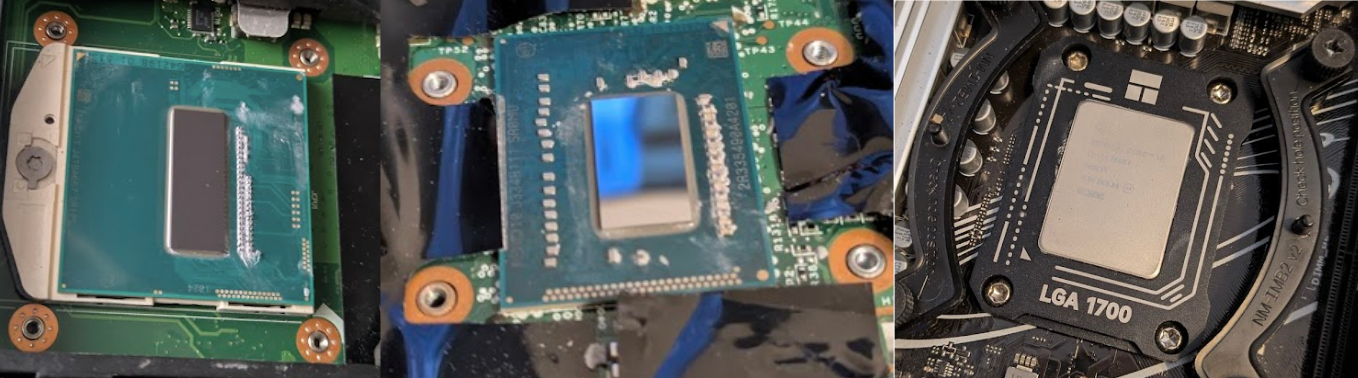
\includegraphics[width=0.85\textwidth]{cpus.png}
    \caption{An Laptop CPU in a socket, an Intel Core i7-4712MQ, a Laptop CPU directly soldered on the motherboard, an Intel Core i7-3520M, and a desktop Intel Core i7-14700KF.}
    \label{fig:cpus}
\end{figure}

\emph{Extra: The shiny part of the CPU is called the die. The die is filled with extremely dense transistors which are all semi-conductive. The die actually does the processing. For those who wonder, no, you cannot see the individual transistors and registers on the CPU; they are so incredibly small and the parts of the CPU are so incredibly small it is impossible to reverse-engineer its architecture; even with microscopes}.

Here are some important points:

\begin{itemize}
    \item CPU's are also called microprocessors. They are interchangeable.
    \item They carry out all the instructions that your computer must do to work.
    \item They exist in phones, tablets, computers, game consoles, etc.
    \item They are responsible for handling input, calculating results and producing outputs\footnote{Example: Getting the input $5+3$ from the user, calculating the result and giving it back to you. This is oversimplified.}
    \item A CPU is a type of integrated circuit; a large network of transistors in a single unit
\end{itemize}

Inside the CPU, there are many important components that are critical to its function. Figure \ref{fig:vonneumann} and \ref{fig:cpu_vonneumann} shows this. Each section that follows explains each part of the diagram. For information on Memory and I/O (or IO), See section \ref{3:sec:ram} and \ref{3:sec:input_and_output_devices} respectively.

\begin{figure}[H]
    \centering
    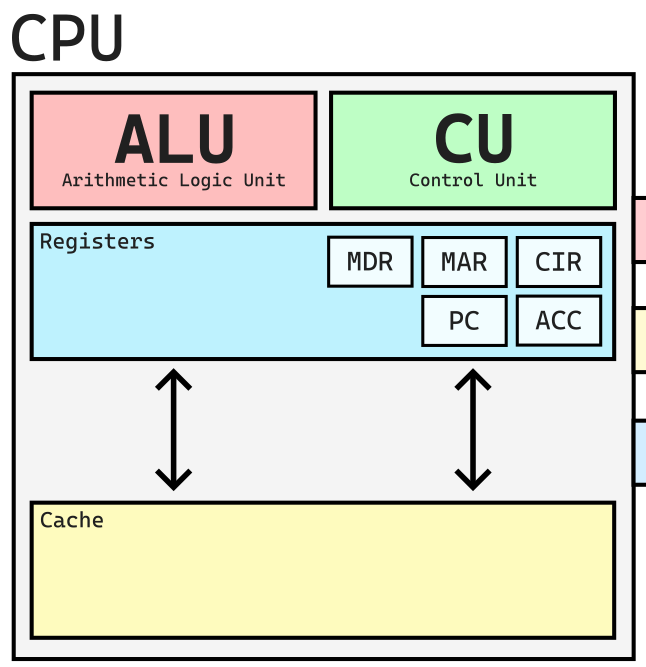
\includegraphics[width=0.4\textwidth]{cpu_vonneumann.png}
    \caption{The CPU on the inside}
    \label{fig:cpu_vonneumann}
\end{figure}

\subsection{The CU, ALU and Registers}

The Control Unit, or CU is like the boss of your CPU. All operations that involve sending data to and from memory or interacting with I/O devices like the mouse and keyboard (refer to figure \ref{fig:vonneumann}) is done by the control unit. It is also responsible for decoding instructions for the CPU to execute.

The ALU or the Arithmetic Logic Unit is responsible for performing all mathematical and logical operations with logic gates, like addition, multiplication and so on, along with AND, OR, NOT, etc.

Registers, like RAM is for fast data storage. The main difference between registers and main memory is that registers are built into the CPU itself. Registers store very little data, typically only 64 bit integers; but are much, much faster than main memory. They also typically serve special purposes. In the diagram, there are 5 important registers that are important for CPU operation.

\begin{itemize}
    \item \textbf{The Program Counter (PC)} is a special register that stores the \emph{address} of the current instruction that is being run by the CPU.
\item \textbf{The Accumulator} is another special register in the CPU that stores intermediate results of arithmetic or logical operations, like the result of $3+5$ or {\ccmono 1 OR 0}. It can accumulate data over time for longer chains of instructions\footnote{In modern CPUs, there is no accumulator. There are so many general-purpose registers that any one can act as an accumulator.}
    \item \textbf{The Current Instruction Register (CIR)} stores the current instruction being executed. This differs from the PC, as the PC stores the \emph{location} of the instruction, whereas the CIR stores the instruction itself.
    \item \textbf{The Memory Address Register (MAR)} stores addresses in memory that must be read from or written to.
    \item \textbf{The Memory Data Register (MDR)} stores the data that must be read from or written to memory. This differs from the MAR, as the MAR stores \emph{locations} (addresses), whereas the MDR stores the locations themselves.
\end{itemize}

General purpose registers also exist, which are registers that can be used for anything.

\paragraph{Extra for experts}

The von neumann architecture in this syllabus is covered in a great way, but this does not reflect modern computers. For instance, there are many more special registers in a modern computer. For a CPU architecture called {\ccmono aarch64} or {\ccmono arm64} (very popular; used in Apple Macs, phones and some game consoles), there are a few more\footnote{This may be specific to aarch64, but other architectures have them too.}

\begin{itemize}
    \item \textbf{The Stack Pointer (SP)} stores the location of the stack. The stack is where large-sized variables are stored in code; it is slower but more flexible than registers as it can hold more data. The stack pointer stores where this continuous chunk of memory begins.
    \item \textbf{The Link Register (LR)} stores the address of the last executed instruction before a branch. Branches are instructions that tell the CPU to go to a specific location to execute instructions, then go back. Before the program counter is set to where the new instructions are, the link register is set so that the CPU knows where to return to after executing the branch.
    \item \textbf{The Current Program Status Register (CPSR)} stores important information about instruction results. After, let's say a comparison (such as {\ccmono 5 > 3}), the result is stored in the CPSR. Then, later instructions read it to execute conditional branches (if statements in code).
\end{itemize}

\subsection{Cache}

Cache simply stores commonly used data and instructions. If there are many similar operations in a row with similar results, the operations themselves and the results of them are put in cache. This means that similar calculations do not have to be done over and over again, instead it is stored in cache (or cached).

Cache is made of SRAM and is inside the CPU, therefore it is fast (faster than RAM!)

\subsection{Buses}

Buses\footnote{For the brits, Busses} are channels by which data flows. Refer to figure \ref{fig:vonneumann} for details.

There are 3 buses to speak of in the von neumann architecture:

\begin{itemize}
    \item \textbf{The Address Bus} is the channel for memory addresses. When the CPU wants to read something from memory, the address is transmitted through the address bus. It is unidirectional, meaning that it is only between the CPU and RAM. It is as wide as memory addresses can be. On modern computers, this is 64 bits wide, or 8 bytes.
    \item \textbf{The Control Bus} is the channel for control signals. It carries signals from the control unit to memory and/or input and output devices (via the I/O controller, pictured in the diagram). These signals are for the CPU, Memory and I/O to coordinate and cooperate. An example could be the CPU telling the RAM that it wants to read data, or telling I/O that it wants to send data to a device. The bus is only 8 bits wide usually, as these only pass simple signals. It is bidirectional, meaning that data goes both ways.
    \item \textbf{The Data Bus} is the channel for actual data. Data that the keyboard sends to the CPU, or data that the CPU sends to memory for writing, like numbers. It is bidirectional for both reads and writes, and the width of the data sent depends, ranging from 8 bits (usually) to 64, or even higher in newer architectures.
\end{itemize}

\subsection{The Fetch-Decode-Execute Cycle}

The fetch-decode-execute cycle is the cycle that the CPU follows to execute instructions over and over again. The cycle itself is as follows:

\paragraph{Fetch}

Is when the CPU gets the next instruction to run from memory. \emph{The instruction at the program counter ends up at the current instruction register}. In terms of the busses,

\begin{itemize}
    \item The CPU places the program counter's value on the \textbf{address bus}, because it's an address.
    \item The CPU sends a read signal to memory over the \textbf{control bus}, to read the data at the address.
    \item Memory responds by sending the instruction at the program counter over the \textbf{data bus}
    \item The data is caught in the current instruction register.
\end{itemize}

\paragraph{Decode}

The instruction is decoded in the control unit.

\paragraph{Execute}

The control unit executes the instruction. For arithmetic instructions and comparisons, it is sent to the ALU. For memory-related instructions, data is sent to and from memory via the CU and the buses.

There is a great video by Tom Scott on this, watch it \href{https://www.youtube.com/watch?v=Z5JC9Ve1sfI}{here.}

\subsection{The Clock Speed}

\begin{figure}[H]
    \centering
    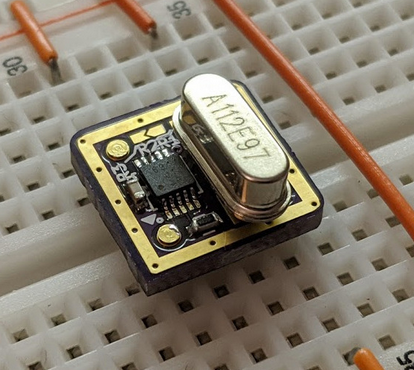
\includegraphics[width=0.4\textwidth]{crystal_clock.png}
    \caption{A crystal clock generator, which generates electrical pulses.}
    \label{fig:crystal_clock}
\end{figure}

The clock speed is the rate at which the Fetch-Decode-Execute cycle is ran at. Figure \ref{fig:crystal_clock} shows a crystal clock generator, which generates electrical pulses. On each pulse, the CPU does either a fetch, decode or execute. Fetches and Executes may take more than one pulse to run, but simply assume each stage takes one pulse.

Since this describes an event that happens regularly, we use hertz (times per second) to measure this. In modern computers and phones, CPUs tend to run at around 3.5 to 4.5 Gigahertz, which means 3.5 billion to 4.5 billion fetches/decodes/executes per second, which is very fast.

\subsection{Cores}

Cores are like Sub-CPUs in each CPU. Each CPU shown in figure \ref{fig:cpus} has more than 1 core. Each of them can carry out tasks independently of each other; despite how they can communicate together. For those who have already read this whole section, each core can carry out its own fetch-decode-execute cycle.

\begin{figure}[H]
    \centering
    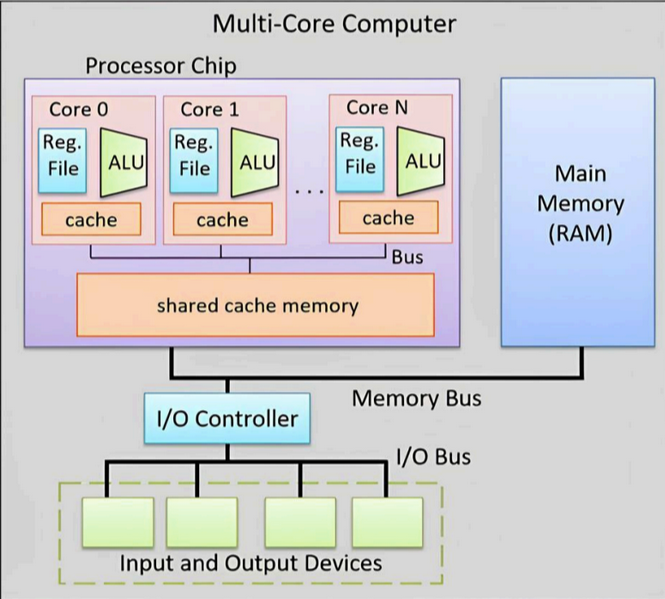
\includegraphics[width=0.7\textwidth]{cores.png}
    \caption{A diagram showing what cores look like in a CPU.}
    \label{fig:cores}
\end{figure}

Each core talks to each other, and every core can communicate with every other core. They are bound together tightly in the CPU; knowing exactly how they communicate is not a part of the syllabus and is too complicated to break down.

There are some special names for multi-core CPUs with lower core counts. \textbf{Quad core CPUs} have 4 cores. \textbf{Dual core CPUs} have 2 cores. \textbf{Single core CPUs} have 1 core, as per the name.

\subsection{Increasing CPU speed}

There are 3 ways:

\begin{enumerate}
    \item \textbf{Increasing the clock speed} increases the amount of F/D/E cycles run per second, meaning more can be done per second; implying a faster chip.
    \item \textbf{Increasing cache} means that more common instructions and their results can be stored at one time, preventing constantly recalculating these instructions.
    \item \textbf{Increasing the amount of cores} means that there are more units that can run the F/D/E cycle per second, meaning more things can be done concurrently.
\end{enumerate}

\end{document}
